\documentclass[12pt,twoside,notitlepage]{report}
\newcommand{\fxch}{FixCache }
\usepackage{a4}
\usepackage{verbatim}
\usepackage{amsmath}
\usepackage{color}
\usepackage[T1]{fontenc}
\usepackage[dvipsnames]{xcolor}
\usepackage{listings}

\usepackage{graphicx}
\graphicspath{ {figs/} }

\title{Dissertation notes}
\author{Tamas Sztanka-Toth \\ ts579@cam.ac.uk}
\raggedbottom                           % try to avoid widows and orphans
\sloppy
\clubpenalty1000%
\widowpenalty1000%

\addtolength{\oddsidemargin}{6mm}       % adjust margins
\addtolength{\evensidemargin}{-8mm}

\renewcommand{\baselinestretch}{1.1}    % adjust line spacing to make
                                        % more readable

\begin{document}
\lstset{language=Python, tabsize=4, backgroundcolor=\color{White}, keywordstyle=\color{blue}, numbers=left}
\setcounter{page}{1}
\pagenumbering{roman}
\pagestyle{plain}
\bibliographystyle{unsrt}
\maketitle{}
\tableofcontents
\cleardoublepage        % just to make sure before the page numbering
                        % is changed

\addcontentsline{toc}{chapter}{\listfigurename}

\listoffigures
\cleardoublepage
\setcounter{page}{1}
\pagenumbering{arabic}
\pagestyle{headings}
\chapter{Introduction}
\section{Motivation}
aaa
\section{Aims of the project}
\cleardoublepage
\chapter{Preparation}
\section{Overview of \fxch algorithm}
\subsection{History and idea}
\fxch is a bug-prediction algorithm implemented in 2007 by researchers at MIT\cite{FixCache}. The original algorithm was implemented for Subversion and CVS, whereas my implementation is for Git. These Source Code Management systems differ in lot of aspects, the key difference between Git and the others, is that Git is distributed, that is it does not require a central 'parent' or 'master' repository. This means that we do not need a remote server access every time we want to commit a new change, we simply commit them locally, and later we can push those commits to a remote location. This feature speeds up programming, but also it introduces new problems to tackle when one is mining repositories\cite{Git}.

The algorithm itself is called \fxch as it uses a notion of a cache, which stores a subset of files in a repository. Following this logic, the algorithm defines a notion of locality: spacial, temporal, new-entity and changed-entity. We use these localities to put files into the cache, to increase its accuracy. As the number of files in the cache (the cache-size) is fixed, we need to take out files from the cache if the cache is polluted. There exist different cache replacement policies\cite{FixCache}:
\begin{itemize}
\item \textit{Least-recently-used (LRU)}: When removing files from the cache we first remove those which were used least-recently. That is they were added/changed earlier in the commit history.
\item \textit{LRU weighted by number of changes (CHANGE)}: This approach will remove files which were changed the least, as the intuition is that more frequently used files are more bug-prone, so we want to keep them in the cache.
\item \textit{LRU weighted by number of faults}: This is similar to the approach before, the only difference is that instead of removing files with least changes it removes files with least faults.
\end{itemize}
In the implementation itself I have used the LRU cache replacement policy, as it is simple, and there is not significant difference between the different replacement policies\cite{FixCache}\cite{Sadowski}\cite{Bugcache}.

The authors argued in the original paper that after \fxch is ran for a repository (I'll further discover the optimal parameters), the files in the cache will more likely have a bug in the future than those which are not in the cache. To evaluate the algorithm self the used a notion of \textit{hit-rate} which can be defined as \[hitrate = \frac{\#hits}{\#hits\ +\ \#misses}\].
I'll discover later what do these exactly mean.
\subsection{Abstract view of the algorithm}
The algorithm works as follows:
\begin{enumerate}
	\item Preload the cache with initial items (new-entity locality).
	\item For each commit C in the repository, starting from the first commit:
	\item If the commit is a fixing commit:
		
	For each file uploaded by that commit, we check if they are in the cache. If a file is in the cache, we record a hit, else we record a miss.
	\item For each file $F$ which were not in the cache, we go back to the commits when the bugs in those files were introduced (say revision $n$), and take some closest files to $F$, at revision $n$ (spacial locality).
	\item We select some subset of new-files and changed-files at C, and put this subset to the cache (new-entity locality and changed-entity locality).
	\item We remove those files from the cache, which were deleted at C (clean-up).
\end{enumerate}
So far, files were only added to the cache. What happens is that the algorithm in the background takes care of cache pollution, and removes files from the cache (LRU) to make space for new arrivals.
\subsection{Hits, misses and hit rate}
We only look-up the cache at so-called bug-fixing commits. To flag a commit as a bug-fixing one, we use a set of regular expressions and parse the commit message. If a message matches any of our regular expressions, it is a bug-fixing commit (following the idea used in \cite{KimZim}).

At each bug-fixing commit, for each file involved in that commit, we make a lookup in the cache. If a file is already in the cache, we note a hit. Otherwise we score a hit. Then we define hit-rate, as mentioned before, as the ratio of hits over all lookups. Since at each commit we either increase the hit-count or miss-count (or both), the hit-rate itself is a cummulative indicator of how good our algorithm is. 

At each commit, the cache contains both fault and non-faulty files. What is really important in \fxch, isthat only truly faulty files score hits, so there is a relation between the hit-rate and True-positives (files that are faulty and are in the cache) in the cache itself, that is there is a relation between hit-rate and the number of identified faulty files. Some might argue that this evaluation strategy is poor, as it is not known what is the window of our prediction, that is how early/late will the files in the cache contain bugs. There exists other, more sophisticated evaluations, by other authors such as \cite{Sadowski} and \cite{Bugcache}.
\subsection{Cache-localities and variables}\label{variables}
As mentioned before there are four different localities when talking about \fxch: temporal, spatial, changed-entity and new-entity. 
\subsubsection{Temporal-locality}
As with physical caches, temporal-locality in \fxch is used following the idea that files which were used (had a fault) will be used (will have a fault) in the near future. At each bug-fixing commit, we load all the files involved in the cache, regardless of whether we recorded a hit, or miss for them.
\subsubsection{Spatial-locality}
Again, the idea of spatial-locality comes from the world of physical caches: when a file is used (has a fault) it is likely that other files "near" to that file will be used (will have a fault). To define nearness, we first need to define the notion of distance for two files in \fxch. Distance is for any two files $f_1$ and $f_2$ at revision/commit $n$ is defined as (following \cite{FixCache}):
\[
	distance(f_1, f_2, n) = \frac{1}{cooccurrence(f_1, f_2, n)}
\]
The $coocurrence(f_1, f_2, n)$ returns an integer: how many times were the files $f_1$ and $f_2$ used (committed) together from revision $0$ to revision $n$.

\textbf{Distance-to-fetch (block-size)}: this parameter (variable) is used to define how many files will be fetched when loading the closest files to a file at revision $n$.

This locality is used every time we have a cache-miss. If a file (say $f_t$) is missed during a bug-fixing commit, we go back to the bug-introducing commit(s) and fetch the closest files to $f_t$ at each bug-introducing commit identified. We can identify the bug-introducing commits using the SZZ algorithm\cite{SZZ}.
\subsubsection{Changed-entity-locality and new-entity-locality}
At each revision we put newly encountered files into the cache. These can be further divided into two categories: new files (new-entity-locality) and files changed between the revision viewed and the previous revision (changed-entity-locality). 

\textbf{Pre-fetch-size}: this variable is used for both changed-entity and new-entity locality to specify how many files should be fetched. At each revision files with higher Lines-of-code (LOC) are put in the cache first. That is if the pre-fetch-size is 5, than we will load at revision $n$ the 5 files with highest LOC.

\subsubsection{Initalising the cache}
To encounter a small amount of misses at the beginning, we need to pre-load the cache with some files at revision $0$. This is done by using the new-entity-locality: each file is new, so each file is considered, and we will load files with the highest LOC, according to the pre-fetch-size, discussed above.
\subsubsection{Cleaning-up}
At each revision we remove the deleted files from the cache, to save space for further insertions and to avoid having false data.
\section{Git}
\subsection{Overview}
Git\footnote{https://git-scm.com/} is a modern code version-control system which uses distributed revision-control. The main difference with other version-control systems, say Subversion is, that Git is fully distributed. That is, a developer can make some changes on their own machine, and without accessing the main repository they can commit their changes to the local machine, as the local machine will have a valid Git repository. Later the developer can push changes from the local repository to the main repository. This approach makes it easier to develop software when internet connectivity is poor, but introduces other issues, such as merge-conflicts. It was developed to help the Linux kernel developers with proper version control system. Since its development in 2005, it has been widely used by open-source projects as their primary VCS. It has a simple design, it is fully distributed and supports non-linear development through branching.
\subsection{Git snapshots - how does the version control works}
Git stores data differently to other major VCSs. Rather than storing for each file the list of changes, git stores the whole repository at each revision point in the history. For efficiency if a file hasn't been changed at a commit, rather then storing the file again, Git only stores a pointer to the last identical file in the previous revision. We can think of a Git repository as an ordered list of snapshots. To view differences (using the git diff command) Git looks up the differences in a repository between two snapshots. In this definition, version control is simply done by storing (committing) at various times the state of our repository, directory structure.
\subsection{Git File structure}
At each revision point in git we can think of data represented by git as a small file structure. Objects in a Git snapshot can either be blobs or trees. Blobs correspond to files whereas trees correspond to directories and subdirectories under the repository. At each point in the history of the repository Git stores a commit object, which stores the meta-data about that commit, for example: the author, the time committed. Furthermore, this commit object has pointer to a tree object, which is the root directory of the repository. Further, each tree can have a pointer to many more trees or blobs. Blobs, as they correspond to file, do not have any children. Each commit has a pointer to it's parent(s), except the initial commit which doesn't have parent(s).
\subsection{Branches in Git}\label{gitbranches}
Branches are an important feature of Git. They allow a non-linear development in a decentralised manner, meaning that developments can make their own changes locally, and later join/merge these changes together. As each commit is simply an object with some meta-data, which stores a pointer to a snapshot, a branch is simply a pointer to one of these commits. The branch named "master" is the default branch (although this can be changed), after initialising a repository you are given a "master" branch which will store a pointer to the latest commit made. When you create a branch, what really happens is that Git creates a new pointer to the commit you are viewing at that moment. Git knows which branch you are on at any time by storing a special pointer called "HEAD" which is a pointer to the branch object you are viewing. It is possible to diverge two branches, that is starting from a commit C, make some changes on branch B1, and later switch to branch B2 and make some changes again on top of C. This was the first commits after C on B1 and on B2 will have the same parent, C, and they will be diverged. Following this logic, you can also merge two branches, that is for example include the changes (that is the set of commits) made on branch B1 to the changes made on B2. If B1 and B2 are on the same linear path, we can simply fast forward, that is point the pointer of B1 to the same place when B2 is pointing. Otherwise, we need a real merge, which can be tricky to do automatically. There are two cases here:
\begin{enumerate}
\item There are no merge conflicts. This means that there is no single file which were changed/overwritten on both branches. In this case Git will handle merging automatically through a so-called "recursive-merging" algorithm.
\item There are merge conflicts. This means that there is at least file which has been modified by both branches B1 and B2. In this case Git will merge the files that it is able to merge, and for those where the conflict arose it will place some readable text to tell the user where the conflict is. The user will have to manually go to each file and resolve the conflict, and commit the new changes later. There exist automated tools for merge-conflict resolution, which automate the last two steps during the merging command itself, but I personally find them quite unintuitive to use.
\end{enumerate}

When a merge occurs Git will create an automated merge commit, which will contain the information about the which commits were merged together, that is this commit will have at least two parents. The changes contained by a merge commit are also visible on the branch they were really made, this is an important feature if you want to view the repository as a linear history of commits. 

As each commit can be a parent of one or more commits and similarly each commit can have zero ore commits we can treat the history of a repository as a Directed Acyclic Graph (DAG). This is a big difference between other VCS softwares as in non-distributed VCS branching is harder to achieve, and once we have it it is quite hard to backtrack which branches were used by which user and when[need better explanation+reference here]. The DAG representation comes handy when analysing different user activities, but it introduces several new problems, because when we are mining a repository we might want to check each path in a repository. 

It is also possible to view each branch as a linear set of commits (even when some branches were merged into this branch). Commits will appear in their order of committed time, regardless on which branch were they made. This linear representation will also contain all the merge commits, which will be the ones with at least two parents. This means, that when going through this history merged changes will be visible twice: once in their original commit (made on some branch B1) and once in the merge commit of branches B1 and B2 say.
\subsection{Git diff with and without the --stat flag}
The command git diff outputs the difference between two snapshots (commits for instance). Without any flags/options set it will output the line-by-line difference with some metadata at the beginning for each file. If the task is only to get the basic information of how files changed it is good to use the --stat flag. With this Git will only outputs which file has had lines deleted and/or added, and how many lines this was. This second is more efficient in the background, due to how diff is implemented (reference here??).
\section{GitPython}
\subsection{Overview}
GitPython\footnote{https://github.com/gitpython-developers/GitPython} is a python package developed by Sebastian Thiel\footnote{https://github.com/Byron} as a purely python high-level tool for interacting with Git repositories. By using it, one is able to do everything via Python: create new repositories, commit changes, checkout branches etc. Each Git object has its own representation in GitPython, and each object is stored in a object database to achieve lower memory overhead. In fixcache, GitPython will only be used to access for the following tasks:
\begin{itemize}
\item Getting the list of commits (for the \texttt{master} branch) in chronological order
\item To determine differences in files between two commits
\item To keep track of each files history: number of changes, faults and lines at each commit.
\end{itemize}
\subsection{The object database}
Behind the scenes: gitdb\footnote{https://github.com/gitpython-developers/gitdb}
Behind the scenes GitPython is using gitdb for accessing a git reposiotry. This is an efficient way of accessing data, as gitdb only operates on streams of data rather than the whole objects, so it actually requires small amount of memory. There are two options here, either we use the defaut \texttt{GitDB} (implemented by the gitdb package) or the \texttt{GitCmdObjectDB} which was only added to the GitPython. The first one, according to the Thiel \textit{"uses less memory when handling huge files, but will be 2 to 5 times slower when extracting large quantities
small of objects from densely packed repositories"} while second one \textit{"uses persistent git-cat-file instances to read repository information. These operate very fast
under all conditions, but will consume additional memory for the process itself. When extracting large files, memory
usage will be much higher than the one of the \texttt{GitDB}"}. Since we \fxch both handle large files and they both extract large quantities of data, I have deduced that it doesn't really matter which one I use, so I went for the default one. This deduction was also supported when comparing the two with real running-time analysis, in fact I found using \texttt{GitCmdObjectDB} is slightly slower when compared to \texttt{GitDB}.
\cleardoublepage
\chapter{Implementation}
\section{Design overview}

The algorithm is implemented in Python using its 2.7.6 release. The implementation has several modules which handle different parts of the algorithm. The three biggest modules are: \texttt{filemanagement}, \texttt{cache} and \texttt{filemanagement}. 

The first implements a layer for representing files, file-sets and distances between files. All these data structures are used by the \texttt{cache} and \texttt{repository} modules. 

The second only contains the \texttt{Cache} class which represents our cache when running \fxch in our \texttt{repository} module. Instances of this class will store how good the algorithm is, that is they will keep track of number of hits and number of misses. Also they will handle file additions, and removals when the cache is filled.

The last one has several classes subclassing the \texttt{RepositoryMixin} class. These are high level classes, all of them use GitPython's \texttt{git.Repo} class for communication with Git repositories. All of them implement a \texttt{run\_fixcache()} method, which will run the fixcache for the given subclass of \texttt{RepositoryMixin} with the parameters set at the time of calling the method. 

Apart from these three modules, there exists two smaller ones: \texttt{parsing} (implementing all kinds of parsing methods used by the above three core modules) and \texttt{helper\_functions}.
\section{Back-end modules}
\subsection{Parsing module}\label{parsing}
This module is responsible for three key things: identifying which lines were deleted in the previous commit (the \texttt{get\_deleted\_lines\_from\_diff} method), identifying which lines in a file are "important" (the \texttt{important\_line} method) and finally for identifying and flagging commit messages as "bug-fixing commits" (the \texttt{is\_fix\_commit} method).
\subsubsection*{The \texttt{important\_line} mehtod}
The SZZ\cite{SZZ} algorithm for identifying which lines have introduced a bug will flag lines without looking more closely what is the content of each line. This was the major criticism of the algorithm itself, proposed by Kim and their colleagues\cite{KimZim}. They proposed several improvements, out of which this method is responsible for checking if a line is blank/empty or if it is a comment line. All such lines are ignored by the algorithm, as it is assumed they did not contribute to the fault introduced. It simply parses each line, and checks whether it is or if it starts with \texttt{\#} (the comment symbol in python). Multi-line comments are ignored, as python uses the same syntax for them and for mutli-line strings.
\subsubsection*{The \texttt{get\_deleted\_lines\_from\_diff} mehtod}
An essential part of the \fxch algorithm is identifying which lines were removed between two revisions. This information is later used when identifying the so-called "bug-introducing" commits.

This method will accept the diff message (produced by the \texttt{git diff} command) for each file, and will return a list of line numbers which were deleted between the two diff-ed revisions. It is a pretty straightforward parsing, as the output of \texttt{git diff} is well-formatted and fairly easy to understand.
\subsubsection*{The \texttt{is\_fix\_commit} method}
For each commit looked at, we need to decide whether it is a fixing-commit or if it is a normal (non-fixing) commit. To identify these commits, we need to parse the commit message itself. If the commit message is accepted by any of the following regular expressions (following \cite{Sadowski}), we flag it as a bug-fixing commit. Regular expressions to look for (presented as Python code) when parsing each commit message:
\begin{itemize}
\item \texttt{r'defect(s)?'}
\item \texttt{r'patch(ing|es|ed)?'}
\item \texttt{r'bug(s|fix(es)?)?'}
\item \texttt{r'(re)?fix(es|ed|ing|age\textbackslash s?up(s)?)?'}
\item \texttt{r'debug(ged)?'}
\item \texttt{r'\textbackslash\#\textbackslash d+'}
\item \texttt{r'back\textbackslash s?out'}
\item \texttt{r'revert(ing|ed)?'}
\end{itemize}
\subsection{File-management module}
When running \fxch we need to somehow keep track of the files we looked at so far, and how many faults and/or changes they had, and what is their LOC. We need to do so, as the cache replacement policies later use this data to decide which file will be removed from the cache, when the cache is full and new files arrive.

Another important problem is to handle the distance between files at each revision. That is, a good implementation would be able to tell for any two files $f_1$ and $f_2$ that what is their co-occurrence (which is reversely proportional to their distance) at any commit $n$.

Both of these problems are handled by the \texttt{filemanagement} module which servers as a back-end for any file-related operation that \fxch use. It has four major classes: \texttt{File, FileSet, Distance} and \texttt{DistanceSet}.

All of these classes implement a \texttt{reset} method, which is called each time we are re-running \fxch with different variables. For all implementations it basically sets each internal class variable to their initial value. This is done, so that we do not need to create a new objects for each and every running of \fxch, so we will create only one object per each file hence we will save space.
\subsubsection*{The \texttt{File} class}
Each file found in our Git repository used by \fxch is represented by a \texttt{filemanagement.File} object. In the implementation we can treat the path for each file as a unique identifier. This means, that when a file is renamed, the implementation treats that as two separate actions: file $f_1$ with path $path_1$ was deleted, and then file $f_2$ with path $path_2$ was added, where $path_1 \neq path_2$. All these file paths are relative to the parent directory of the repository itself, rather than absolute paths. This class has three basic functions:
\begin{itemize}
\item \texttt{changed(self, commit)}: Called when a file has been changed, at a commit $c$ (where $c$ is an integer, representing the order of a commit, rather than its sha1 hash).
\item \texttt{fault(self, commit)}: Similar to \texttt{change}, but called when a file has a fault fixed, that is at any bug-fixing commit. It needs to be called together with \texttt{change}.
\item \texttt{reset(self, line)}: Resets a \texttt{File} object.
\end{itemize}
\subsubsection*{The \texttt{FileSet} class}
We can think of this class as a memory-stored database, which stores \texttt{File} objects. We can query a \texttt{FileSet} object (via the path of a file) and it will return the object corresponding for the file with that path. The method \texttt{FileSet.get\_or\_create\_file} (which accepts a path, and several other variables as input) will do exactly this: it looks at the internal \texttt{FileSet.files} dictionary, and if the path we are looking for is present, it will return the value for that path. Otherwise, it will create a new file with that path, and return the newly created file.

The function which is actually used by the \texttt{repository} module is the \texttt{FileSet.get\_and\_update\_multiple} method. This, rather than accepting a single path to a file, accepts the output of the \texttt{git diff --stat} command, which for example looks like this:
\begin{verbatim}
setup.py | 11 ++++++++++-
 1 file changed, 10 insertions(+), 1 deletion(-)
\end{verbatim}
Luckily we do not need to parse this, as GitPython already has a parser, which will parse it and create a nested Python dictionary. For the output above, this dictionary will look like this:
\begin{verbatim}
{u'setup.py': {'deletions': 1, 'lines': 11, 'insertions': 10}}
\end{verbatim}
Each changed file's path will be a key in this dictionary, and the corresponding value will be an another dictionary with three keys: \texttt{deletions, lines, insertions}. 

Our function will use this parsed \texttt{diff} data to keep track of number of lines in each file (as $linechange = insertions - deletions$), when the files were added, when the files were changed (if they already existed in our \texttt{FileSet} instance, and when they are deleted. We assume that each file is deleted when their LOC (lines-of-code) becomes zero.

After updating the data for each file and creating new files, it will return a list of tuples, where the second value of a tuple will be the actual \texttt{File} instance, and the first value will be either \texttt{'changed'} or \texttt{'deleted'} or \texttt{'created'} dependant on what happened to that file between the \texttt{diff}-ed commits we are viewing.
\subsubsection*{The \texttt{Distance} class}
In order to implement the temporal-locality used by \fxch we need to know the co-occurrence of any two files at any commit. To do that, for each two files committed together a \texttt{Distance} instance will be created. This instance will have a list of commit numbers representing the commits when the two files were changed together. That is, for each two files in a commit, we either update the corresponding \texttt{Distance} object, or we create a new one if it has not yet existed.
\subsubsection*{The \texttt{DistanceSet} class}
The previously described \texttt{Distance} class is not directly used by our \texttt{repository} module. It merely serves as a back-end representation used by a \texttt{DistanceSet} object, which will interact with the \texttt{repository} module. This class stores a dictionary for \texttt{Distance} object: we generate a key for each pair of files, and as a value for that key we store their \texttt{Distance} instance. 
\paragraph{Key generation} The key generation is fairly simple: we look at which file's path is 'smaller' (that is would come earlier in an English dictionary) and append this path to the 'bigger' path. That is:
\begin{gather*} 
	\forall f_1, f_2\ files \\
	key(f_1, f_2) = \begin{cases}
						f_1.path+f_2.path &if\ f_1.path > f_2.path\\
						f_2.path+f_1.path &if\ f_1.path < f_2.path\\
						error &otherwise: two\ paths\ equal, f_1 == f_2
					\end{cases}
\end{gather*}
\paragraph{Important functions}
\begin{itemize}
\item \texttt{get\_occurrence(self, file1, file2, commit=None)}

Accepts two files and a commit (the commit's integer representation, a counter) as an input, and outputs their co-occurrence (a non negative integer) before, and including the commit. If the \texttt{commit} argument is none, it simply outputs the current, known co-occurrence of the two files. For the \texttt{Distance} object for the two input files, it looks at the commit list, and counts the commits which are smaller (happened earlier) or equal to the input commit.
\item \texttt{add\_occurrence(self, file1, file2, commit)}

For two files, add the commit number (again, an integer) to the \texttt{Distance} object of the two files.
\item \texttt{get\_closest\_files(self, file\_, number, commit=None)}

For a single file \texttt{file\_}, look at all \texttt{Distance} objects in which \texttt{file\_} is present. For these objects, calculate the co-occurrence, and return the top \texttt{number} of files.
\item \texttt{remove\_files(self, files)}

Removes all the \texttt{Distance} instances which contain any of the input \texttt{files}. That is: go through each file in the input \texttt{files} list, and delete all \texttt{Distance} objects which have this file.
\end{itemize}
\subsection{Cache implementation}
\fxch uses the notion of a file cache, which has some limited number of files in it. We can think of it as a bucket, where we can put some files in, and when the bucked is filled, it will automatically take care of cleaning up some other files in order to make space for new arrivals. The \texttt{Cache} class is responsible for keeping track of files which are in the cache, counting hits, counting misses and removing files (according to or LRU policy).	
\paragraph{Core methods}
\begin{itemize}
\item \texttt{\_remove\_multiple(self, number=1)} 

Remove \texttt{number} number of files from the cache, according to the LRU cache-replacement policy.

\item \texttt{add\_multiple(self, files)}

Add multiple files into the cache. If there is not enough space,  the above mentioned method will be called in order to make space for the arriving files. If we want to put in too many files (ie the cache size is smaller than the number of arrivals) we pre-process the arriving files by selecting the most recently used, to obey LRU.

Similarly there exists methods for adding and removing a single file from the cache: \texttt{\_remove(self)} and \texttt{add(self, file\_)}. 

Only addition methods are called explicitly by the \texttt{repository} module, all the removing methods are only called implicitly when calling additions.
\end{itemize}
Internally, files are stored in Python's \texttt{set()} object, which does not allow duplicates, but it does not have by default a limit. To actually have a limit in our cache implementation, all addition methods first look up how many files are currently in the cache, and subtract that value from the cache size to get how big is the currently available space. Removing files works accordingly to this: if we need more space, we remove as many files as necessary to get it.
\section{Core algorithm implementation}
\subsection{Identifying fixing commits: the SZZ algorithm}
The SZZ algorithm was introduced by J. \'Sliverski, T. Zimmermann and A. Zeller \cite{SZZ}. This algorithm tries to identify which commit introduced a bug in a file, when viewing the file at a fixing-commit. The algorithm roughly works the following way:
\begin{enumerate}
\item At a fixing commit, identify which lines were deleted at this between this commit and it's parent commit. We assume that all of these lines were deleted as a result of the bug-fixing procedure, so that they contributed to the bug itself.
\item Once we know the lines, we need to check where were these lines introduced. We take all these commits, and say that these are the bug-introducing commits for a given bug-fix. In Git, getting which lines were introduced by which commit is quite straightforward using the \texttt{git blame} command.
\item Do steps 1-2. for each bug-fixing commit.
\end{enumerate}
The assumption made by SZZ, that each deleted line in fact was a 'buggy' line is a really strong one, and it leads to plenty false positive lines. There are several techniques to lower this number, which are discussed in more detail by \cite{KimZim}. Out of those, as in section \ref{parsing}, this SZZ implementation is only using the comment-line and blank-line reduction.

The SZZ algorithm in this implementation is implemented inside the \texttt{repository.Repository} class, rather than a standalone module, as it is a core part of \fxch. The two functions which are implementing it are:
\begin{itemize}
\item \texttt{\_get\_diff\_deleted\_lines(self, commit1, commit2)}

Returns the deleted line-numbers (per file) between any two commits. Used to get the deleted lines between a commit and it's parent.
\item \texttt{\_get\_line\_introducing\_commits(self, line\_list, file\_path, commit)}

Once we have the line numbers which were deleted between two commits (commit and it's parent) we can for each file get the list of bug-introducing commits. This method uses the \texttt{git blame} (which, in GitPython outputs a nested list, where the first value of a list is a commit object, and the second value is a list of lines last changed - introduced - by that commit), and produces a list of bug-introducing commits.
\end{itemize}
\subsubsection*{Commits which introduced a bug}
We only need to call the SZZ algorithm for bug-fixing commits. To do this, we first need to identify bug-introducing changes. We do this following a different approach that was used in the original SZZ algorithm, as explained earlier in the section \ref{parsing}.
\subsection{The \texttt{Repository} class}
This class is the central element of the \fxch implementation. It is connecting all modules together, and uses them to run and analyse the algorithm for different repositories. The \texttt{Repository} class is inside the \texttt{repository} module, which has two more classes, used only for evaluation purposes. 
\paragraph{Cache size initialisation} Upon initialisation we need to set the variables used by our algorithm. First of all, we need to set the \texttt{cache\_ratio} which will be a real number between 0.0 and 1.0. From the \texttt{cache\_ratio} we calculate \texttt{cache\_size} (which will be the exact number of how many files do we allow in our cache) the following way: we take the number of files in the repository at the last commit, and we multiply this number by the \texttt{cache\_ratio}. We then take the floor of this number (if the floor is zero, we add one, as the \texttt{cache\_size} cannot be zero). That is mathematically:
\begin{align*}
	\forall cache\_ratio \in (0.0\dots 1.0]\\
	cr = file\_count\_at\_last\_commit*cache\_ratio\\
	cache\_size = \begin{cases}
						1 & if\ floor(cr) = 0\\
						floor(cr) & otherwise
					\end{cases}
\end{align*}
To calculate the variable \texttt{file\_count\_at\_last\_commit} we need to traverse the git tree at the latest revision, and count the number of 'blobs' (objects representing files) in the tree. A strong assumption is made here, namely that the repository will always increase as history moves forward. 

\paragraph{Setting variables} Once we calculated and set \texttt{cache\_size} we can calculate other variables, such as \texttt{distance\_to\_fetch} (block-size) and \texttt{pre\_fetch\_size} as discussed in \ref{variables}. In the original paper all these variables are given as a percentage of \texttt{file\_count\_at\_last\_commit}, that is if \texttt{file\_count\_at\_last\_commit = 100} then if \texttt{distance\_to\_fetch = 5\%} means that we will fetch 5 files each time we use our spacial-locality.

Rather than using percentages, in the \texttt{Repository} both \texttt{distance\_to\_fetch} and \texttt{pre\_fetch\_size} are rational numbers between 0.0 and 1.0. Also, they are not ratios of \texttt{file\_count\_at\_last\_commit}, but rather of \texttt{cache\_size}. That is if \texttt{file\_count\_at\_last\_commit = 100}, \texttt{cache\_ratio = 0.1} and \texttt{distance\_to\_fetch = 0.5} then we will fetch $100*0.1*0.5 = 5$ number of files.

A \texttt{Repository} instance also has a \texttt{file\_set} variable set to a \texttt{filemanagement.FileSet} instance and a \texttt{file\_distances} set to a \texttt{filemanagement.DistanceSet} instance. We are using these to keep track of files and distances in our repository. Each time we call \texttt{reset()} on our \texttt{Repository} instance (that is every time we want to re-run an analysis, with different parameters) it will also call the \texttt{reset()} method of \texttt{file\_set} and \texttt{file\_distances}.

\paragraph{Initialising commits} Since in Git each commit's identifier is a 40-digit long hexadecimal number generated by SHA-1, it is impossible to know just from the hash value what is the order of commits. Our \fxch is using integers as commit identifiers (the bigger the commit number, the later it happened), so a \texttt{commit\_order} dictionary is initialised (with the \texttt{Repository.\_init\_commit\_order()} method) when a \texttt{Repository} instance is created. This \texttt{commit\_order} dictionary stores the SHA-1 value for each commit as key, and store their numeric (integer) representation as value. Each time we want to access the order of any commit object, we can lookup this dictionary.
\paragraph{Running \fxch}
To run \fxch we need to call \texttt{run\_fixcache} on any \texttt{Repository} instance; calling this method will run \fxch with the parameters currently set to some value. The idea is, that between two runs we call the \texttt{reset} method to change the internal variables, and the expectation is that with different variables the output will also be different.

Given all other modules the algorithm implementation is straightforward, a pseudo-code would look something like this:
\begin{lstlisting}
cache = Cache(*args, **kwargs)
hits = 0
misses = 0
for commit in commit_list:
	parents = commit.parents
	
	if len(parents) == 0:
		initial_pre_load_cache(cache, commit)
	elif len(parents) == 1:
		if bug_fixing(commit):
			for f in commit.files:
				if f in cache:
					hits = hits + 1
				else:
					misses = misses + 1
					cache.add(f) # temporal-locality
					# get bug introducing commits
					bic = get_bic(f, commit)
					# get the closest files to f at bci: spatial-locality
					cache.add_multiple(get_closest_files(f, bci)
			
			# new-entity and changed-entity locality
			cache.add_multiple(commit.changed_files + commit.new_files)
	else:
		pass

bug_prone_files = cache.file_set
\end{lstlisting}
Cache additions are handled by our \texttt{Cache} instance, while other operations (such as functions implementing SZZ) are handled by internal functions of \texttt{Repository}. This pseudo-code is only an abstract implementation to demonstrate how could be \fxch implemented, in the real implementation these functions do not exist (or exist differently), but the functionality is the same.

In the above example we have two if-statements: firstly how many parents does a commit have. If it has zero, it means that we are viewing the initial commit, so we need to pre-load the cache with some initial files (files with the biggest LOC). If it has one parent we proceed normally. If it has two or more parents it means that we have reached a merging commit, which we can disregard as the changes listed there already have been listed somewhere earlier in our commit history, as discussed in \ref{gitbranches}.

The second if-statement is when we are going through all files in our commit. If the file $f$ was already present in the cache, we increase the hit-count. Otherwise, we increase the miss-count and and this file to the cache (temporal-locality). Furthermore, we identify the commits which introduced (lets say: $bci_1, bci_2 \dots bci_n$ the bug-fixed in this commit, and add the closest files to $f$ at $bci_1, bci_2 \dots bci_n$ (spatial-locality).

Furthermore, for each commit we add the changed and updated files to the cache (new-entity and changed-entity locality). 

All these additions are bounded by some numbers specified by the \texttt{pre\_fetch\_size} and \texttt{distance\_to\_fetch} however these are omitted from the pseudo-code.
\section{Versions}
\clearpage
\section{Implementation difficulties}
\subsection{Using GitPython}
When using 3rd party software it is always key if the software we are using have a good or bad documentation (if it has a documentation at all). I have found that GitPython has generally good documentation, although some pieces (object reference, internal methods and variables of classes) lack proper definitions and clear type descriptions. There were times when the only way of finding out something about a certain class was to dive deep into the source-code of GitPython and try to figure out how is the certain class implementing functionalities provided by Git itself. This resulted in a slow implementation speed at the beginning of this project.
\subsection{Bottleneck}
During one run of \fxch there are several times when we have to select the "top objects from a set of objects". The "top objects" might mean "files with biggest LOC" or "least recently used files" or "closest files to a file at a commit". Usually the order does not matter after selection, we do not care whether the $k$ number of files are sorted after selection, as long as all selected files are "bigger" (ie. "have greater LOC" or "were used least recently" or "are closer than") than any file which was not selected.
\paragraph{Initial implementation}
Initially all these selection algorithms were implemented by: first sorting the whole set of $n$ files, and then selecting the top $k$ elements. This is rather inefficient in two cases:
\begin{enumerate}
\item If $k << n$, then we are wasting time on an $\mathcal{O}(n\log(n)$ operation, while we could do in $\mathcal{O}(n\log(k))$ which would be more efficient.
\item If $k >= n$, then we could just return the whole set of $n$ files, which is $\mathcal{O}(1)$ as the order after selection does not matter, thus we are wasting time again on sorting ($\mathcal{O}(n\log(n)$).
\end{enumerate}
\subsection{Speed-up}\label{gettopk}
To achieve speed-up we need to implement a "select top k elements from n objects" algorithm. Using a binary-min-heap, the pseudo-code looks like this:
\begin{lstlisting}
get_top_elements(objects, k):
	if len(objects) <= k:
		return objects
	else:
		heap = BinaryHeap()
		for item in objects:
			if len(heap) < k:
				heap.push(item)
			elif len(heap) == k:
				if item < heap.get_min()
					pass
				else:
					heap.pop()
					heap.push(item)
		return heap
\end{lstlisting}
We need a heap to keep track of what is the minimal item in the currently selected $k$ objects. If we find anything that is bigger than the current minimum, and if there is no space in the heap (ie. $len(heap) == k$) we pop the smallest item, and insert a new one. The time complexity of insertion and pop operations for a heap of size $k$ is $\mathcal{O}(\log{k})$, and since we need to traverse all the objects, the above function has a time complexity bounded by $\mathcal{O}(n\log{k})$ as required.
\begin{figure}[h]
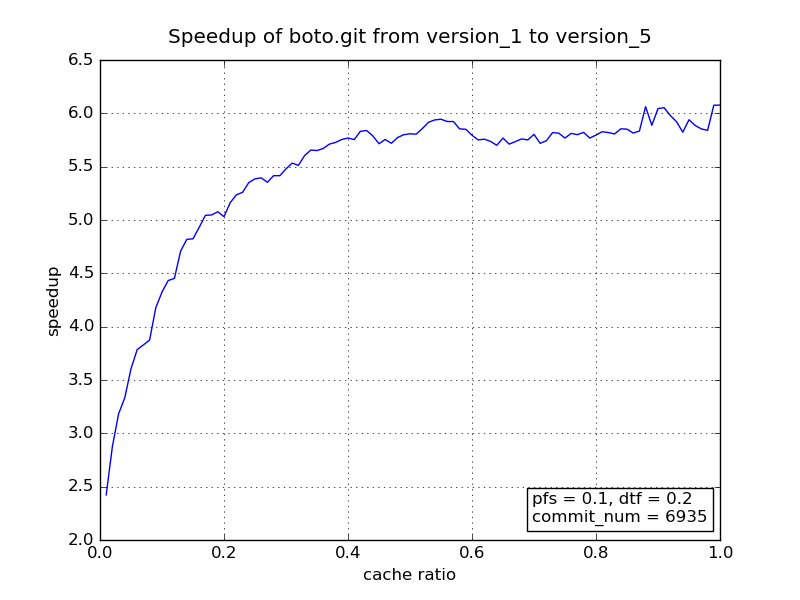
\includegraphics[width=0.5\textwidth]{figure_1.png}
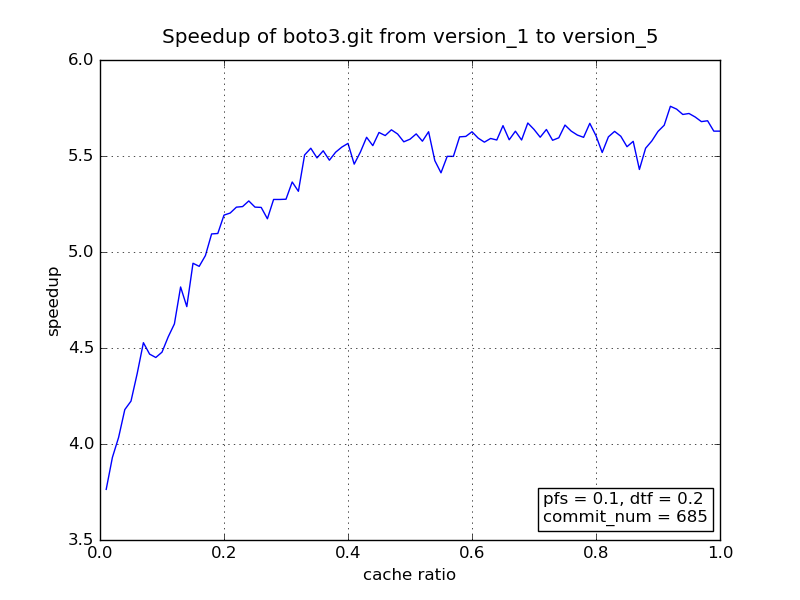
\includegraphics[width=0.5\textwidth]{figure_2.png}

\caption{Speedup of boto.git and boto3.git between version\_1 and version\_5 with different cache-ratios}
\label{fig:speedup}
\end{figure}

We can see on figure \ref{fig:speedup} how good is the speedup for two repositories: on the x-axis we have the cache ratio as a percentage, and on the we have the speedup between version\_1 and version\_5, where we define speedup the following way:
\[speedup(version\_1,version\_5) = \frac{time\_to\_run(version_5)}{time\_to\_run(version_1)}
\]
That is we can see on the left hand diagram of \ref{fig:speedup} that when the cache-ratio is 0.2 version\_5 is 5.0 times faster than version\_1. The reason why speedup increases with cache-ratio is that whenever we increase the cache-ratio we also increase the cache-size. Also, the bigger the cache size, the bigger the pre-fetch-size and distance-to-fetch, so we will fetch more files, hence our "get top k elemens from n objects" algorithm explained in \ref{gettopk} will run in $\mathcal{O}(1)$ time more often, as $k$ (the number of files we are fetching) will increase with $n$ unchanged.
\chapter{Evaluation}
\addcontentsline{toc}{chapter}{Bibliography}
\bibliography{refs}
\end{document}
